\documentclass[aspectratio=169,xcolor={table, dvipsnames}]{beamer}

\usepackage{svg}
\usepackage{graphicx}
\usepackage{tabularx}
\usepackage{booktabs}
\usepackage{tikz}
\usepackage{standalone}
\usepackage{caption}
\usepackage{subcaption}
\usepackage{xcolor}
\usepackage{hyperref}
\usepackage{pgfplots}
\usepgfplotslibrary{fillbetween}

\usepackage[backend=biber]{biblatex}

\addbibresource{2024_ad-fidelity.bib}

\usetikzlibrary{positioning, shadows, fit, backgrounds, overlay-beamer-styles, shapes.arrows, arrows.meta}

% make references tiny, so they don't take up much slides
\renewcommand*{\bibfont}{\tiny}

% modern minimalist latex theme
\usetheme{metropolis}

% fill blocks with background color
\metroset{block=fill}

% footer
\setbeamertemplate{frame footer}{\href{https://github.com/chillerb}{\insertshortauthor}\hfill\insertshorttitle}

%\setbeamertemplate{frame footer}{\insertshortauthor~(\insertshortinstitute)}


\renewcommand{\emph}[1]{\textbf{#1}}

\title[Fidelity of Explanations for AD Classification from MRI]{Evaluating the Fidelity of Explanations for Convolutional Neural Networks in Alzheimer’s Disease Detection}

\author[Hiller]{Bjarne C. Hiller}
\date{2025-03-09}
\institute[Uni Rostock]{University of Rostock}

%\logo{
\includegraphics[height=0.5cm]{logos/logo-uni-hro}}

\titlegraphic{
    \href{https://vac.uni-rostock.de/}{\includegraphics[height=1cm]{logos/logo-vac}}\hfill
    \href{https://www.uni-rostock.de/}{
\includegraphics[height=1cm]{logos/logo-uni-hro}}\hfill
	\href{https://www.dzne.de/}{
\includegraphics[height=1cm]{logos/logo-dzne}}
}

\begin{document}

\maketitle

% \begin{frame}{Agenda}
% 	\tableofcontents
% \end{frame}

\begin{frame}{Motivation}

\end{frame}
% \begin{frame}{Deep Learning for Medical Image processing}
% 	% introduce deep learning and XAI
% 	% - want to analyse MRI from AD subjects
% 	% - Deep Learning powerful for image processing, expert level performance
% 	% - however, Black Box systems
% 	% - Can we trust prediction?
% \end{frame}
\begin{frame}{Data and Preprocessing}
	\begin{columns}
		\begin{column}{0.5\textwidth}
			\begin{figure}
				\documentclass{standalone}

\usepackage{tikz}

\usetikzlibrary{positioning, shadows, fit}

\begin{document}

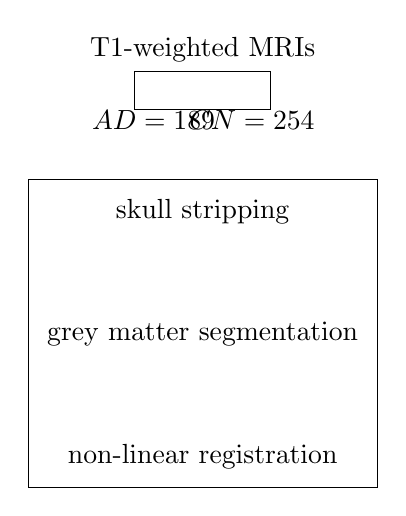
\begin{tikzpicture}
	\node[label=below:{$AD = 189$}] (ad) {};
	\node[label=below:{$CN = 254$}, right=of ad] (cn) {};
	\node[fit=(ad)(cn), label=above:{T1-weighted MRIs}, draw, rectangle] (adni) {};

	\node[below=of adni] (skull) {skull stripping};
	\node[below=of skull] (gms) {grey matter segmentation};
	\node[below=of gms] (im_reg) {non-linear registration};

	\node[fit=(skull)(gms)(im_reg), draw, rectangle] {};
\end{tikzpicture}

\end{document}

			\end{figure}
			%			\begin{block}{Data and Preprocessing}
			%				\vfill
			%				\begin{itemize}
			%					\item $N=443$ ($AD = 189$, $CN=254$) T1-weighted MRI from ADNI database
			%					\item Skull Stripping, Gray-matter segmentation, Non-linear registration (MNI)
			%				\end{itemize}
			%			\end{block}
		\end{column}
		\begin{column}{0.5\textwidth}
			\begin{figure}
				\begin{tikzpicture}
					\node [draw, rectangle, fill=white, drop shadow, inner sep=0] (ttest) {\includegraphics[width=\textwidth]{figures/ttest.png}};
				\end{tikzpicture}
				\caption*{Voxel-wise Welch's $t$-test ($\alpha = 0.01$)}\label{fig:ttest}
			\end{figure}
		\end{column}
	\end{columns}
\end{frame}

\begin{frame}{A CNN Model for AD vs CN Classification}
	\centering
	% 	\begin{block}{Data and Preprocessing}
	% 		\vfill
	% 		\begin{itemize}
	% 			\item $N=443$ ($AD = 189$, $CN=254$) T1-weighted MRI from ADNI database
	% 			\item Skull Stripping, Gray-matter segmentation, Non-linear registration (MNI)
	% 		\end{itemize}
	% 	\end{block}
	\begin{figure}
		\begin{tikzpicture}
			\node [draw, rectangle, fill=white, drop shadow, inner sep=0] (cnn) {\includegraphics[angle=90, width=\textwidth]{tikz/standalone/cnn.tikz/cnn.pdf}};
		\end{tikzpicture}
	\end{figure}
	\visible<2->{
		\begin{columns}[t, onlytextwidth]
			\begin{column}{0.45\textwidth}
				\visible<2->{
					\begin{table}
	\centering
	%\footnotesize
	\rowcolors{2}{white}{gray!25}
	\begin{tabularx}{\textwidth}{XXX}
		\toprule
		AUC ROC         & Accuracy  \\
		\midrule
		$0.95 \pm 0.02$ & $87.64\%$ \\
		\bottomrule
	\end{tabularx}
	\caption*{5-fold Cross Validation Results}\label{tab:cv}
\end{table}

				}
			\end{column}
			\begin{column}{0.45\textwidth}
				\visible<3->{
					\begin{block}{Acceptable Performance...}
						...but can we \emph{trust} the model?
					\end{block}
				}
			\end{column}
		\end{columns}
	}


	%	\begin{columns}[T]
	%		\begin{column}{0.5\textwidth}
	%			\begin{block}{ADNI Data and Preprocessing}
	%				\vfill
	%				\begin{itemize}
	%					\item $N=443$ ($AD = 189$) T1 MRI
	%					\item Gray-matter segmentation
	%					\item Non-linear registration to MNI
	%				\end{itemize}
	%			\end{block}
	%		\end{column}\hfill
	%		\begin{column}{0.5\textwidth}
	%			\begin{block}{Problem}
	%				Can the model be trusted?
	%				\vfill
	%			\end{block}
	%		\end{column}
	%	\end{columns}
\end{frame}

\begin{frame}{Attribution Maps: What did the network look at?}
	\begin{figure}
		\centering
		\begin{tikzpicture}
			\node [draw, rectangle, fill=white, drop shadow, inner sep=0] (cnn) {\includegraphics[angle=90, width=\textwidth]{tikz/standalone/cnn.tikz/cnn.pdf}};
			\visible<2->{
				\node[draw=red, ultra thick, rectangle, anchor=east, minimum width=1.5cm, minimum height=3cm] (outbox) at (cnn.east) {};
				%\draw[draw=red, ->, ultra thick] (outbox.south) -- ++ (0, -1) --++ (-10,0) node[midway, below] {\emph{Relevance Propagation}} node[at end] (backprop){};
				\node[below=0.5cm of cnn.south west, anchor=north west, draw, rectangle, inner sep=0, drop shadow, label=below:relevance map] (attribution) {\includegraphics[height=2cm]{figures/grad-cam-map.png}};
				\draw[draw=red, ->, ultra thick] (outbox.south) |- (attribution.east) node[midway, below, anchor=north east] {\emph{Propagation of Relevance}};
			}
		\end{tikzpicture}
		%\caption*{Attribution of change in model output to change in model input.}\label{fig:attribution}
	\end{figure}
\end{frame}

\begin{frame}[plain]{Why should I care?}
	\centering
	\begin{figure}
		\begin{subfigure}[b]{0.3\textwidth}
			\centering
			\begin{tikzpicture}
				\node[inner sep=0, draw, rectangle, drop shadow] (tinauer) {\includegraphics[height=5cm, trim={0 0 1150px 0}, clip]{figures/tinauer_2022.png}};
				\begin{scope}[overlay, visible on=<2->]
					\draw[<-, red, ultra thick] (tinauer.east) -- ++ (0.5,0) node (pointerstart) {};
					\draw[->, red, ultra thick] (pointerstart.center) |- ++ (-0.5,1.5);
					\draw[->, red, ultra thick] (pointerstart.center) |- ++ (-0.5,-1.7);
				\end{scope}
			\end{tikzpicture}
			\caption{From: \citeauthor{tinauer_interpretable_2022}~\cite{tinauer_interpretable_2022}}\label{fig:tinauer}
		\end{subfigure}\hfill
		\begin{subfigure}[b]{0.7\textwidth}
			\begin{tikzpicture}
				\node[inner sep=0, draw, rectangle, drop shadow] (tinauer) {
					\includegraphics[height=5cm, trim={190px 0 0 0}, clip]{figures/zech_2018.png}
				};
				\begin{scope}[overlay, visible on=<3->]
					\node[red, ultra thick, circle, draw, minimum width=2cm] at (-0.9,1.1) {};
					\node[red, ultra thick, circle, draw, minimum width=2cm] at (4.5,1.5) {};
				\end{scope}
			\end{tikzpicture}
			\caption{From: \citeauthor{zech_variable_2018}~\cite{zech_variable_2018}}\label{fig:zech}
		\end{subfigure}
		\caption*{Attribution maps can reveal \emph{shortcut learning}:  Neural Networks can use features outside of the brain parenchyma (\subref{fig:tinauer}) or X-ray side marker tokens (\subref{fig:zech}) for classification.}
	\end{figure}

\end{frame}

\begin{frame}[plain]
	%{eXplainable AI and Feature Attribution Methods}
	% - explain overall principle of feature attribution methods
	% - plethora of feature attribution methods
	% - Can we trust *explanation*?
	% - "Not sure, if model is broken, or explanation is wrong"
	\begin{figure}
		\centering
		\includegraphics[width=0.9\textwidth]{figures/overview.png}
		\caption*{Popular feature attribution methods for Deep Neural Networks and their Relationships}
	\end{figure}
\end{frame}

\begin{frame}[plain]
	\centering
	\includegraphics[width=0.85\textwidth]{figures/3672-relevance-maps.png}
\end{frame}

\begin{frame}{Total Relevance per ROI}
	\input{tables/rois_total.tex}
\end{frame}

\begin{frame}{Mean Relevance per ROI}
	\input{tables/rois_mean.tex}
\end{frame}
\begin{frame}[plain]
	\begin{center}
		\begin{figure}
			\href{https://knowyourmeme.com/memes/futurama-fry-not-sure-if}{
				\includegraphics[width=0.7\textwidth]{figures/fry-and-xai-2.png
				}}
			\caption*{But can the \emph{explanation} be trusted?}
		\end{figure}

	\end{center}
\end{frame}


\begin{frame}[plain]{Perturbation Tests: Insertion and Deletion}
	% 	% introduce perturbation tests
	\begin{figure}
		%\resizebox{0.5\textwidth}{!}{
		\documentclass[beamer]{standalone}

\usepackage{tikz}
\usepackage{pgfplots}

\usetikzlibrary{positioning, shadows, fit, arrows.meta, backgrounds, overlay-beamer-styles}


\begin{document}
\pgfplotsset{delpoint/.style={
			scatter,
			thick,
			mark=o,
			mark size=5pt,
			only marks,
			scatter,
		}}

% Define style for line plots
\pgfplotsset{delline/.style={
			mesh,
			thick,
			samples=50
		}}

\newcommand{\funcDel}[1]{100 * exp(-3 * #1 / 100)}
\begin{tikzpicture}
	\pgfmathsetmacro{\pointAx}{0}
	\pgfmathsetmacro{\pointBx}{23}
	\pgfmathsetmacro{\pointCx}{100}

	\pgfmathsetmacro{\pointAy}{\funcDel{\pointAx}}
	\pgfmathsetmacro{\pointBy}{\funcDel{\pointBx}}
	\pgfmathsetmacro{\pointCy}{\funcDel{\pointCx}}
	\begin{axis}[
			title={Deletion},
			xlabel={Perturbation Amount},
			ylabel={Predicted Class Probability},
			axis lines=left,
			xmin=-10, xmax=110,
			ymin=-10, ymax=110,
			xtick={0,100},
			ytick={0,100},
			legend pos=north west,
			%ymajorgrids=true,
			%grid style=dashed,
			%yticklabel style={rotate=90}, % Rotate y-axis labels by 45 degrees
			xticklabel=\pgfmathprintnumber{\tick}\%, % Add % sign to x-axis labels
			yticklabel=\pgfmathprintnumber{\tick}\%, % Add % sign to y-axis labels
			colormap={coolwarm}{
					rgb(0cm)=(0,0,1);
					rgb(1cm)=(1,0,0);
				},
			scatter src=y,
		]

		% Define a variable
		%\pgfmathsetmacro{\phi}{3}

		% Define a function
		%\pgfmathsetmacro{\f}{100 * exp(-\phi * x)}

		\only<1>{
			\addplot[delpoint]
			coordinates {
					(\pointAx, \pointAy)
				};
		}
		\only<2>{
			\addplot[delpoint]
			coordinates {
					(\pointAx, \pointAy)
					(\pointBx, \pointBy)
				};
			\addplot[delline, domain=0:23] {\funcDel{x}};
		}
		\only<3>{
			\addplot[delpoint]
			coordinates {
					(\pointAx, \pointAy)
					(\pointBx, \pointBy)
					(\pointCx, \pointCy)
				};
			\addplot[delline, domain=0:100] {\funcDel{x}};
		}


		\node at (axis cs: \pointAx,\pointAy) (pointA) {};
		\node at (axis cs: \pointBx,\pointBy) (pointB) {};
		\node at (axis cs: \pointCx,\pointCy) (pointC) {};

	\end{axis}

	\visible<1->{
		\node[draw, rectangle] at (pointA -| 10, 0) (inputA) {};
		%\node[draw, rectangle,right=5cm of pointA] (inputA) {};
		\draw[->] (inputA) -- (pointA);
	}

	\visible<2->{
		\node[draw, rectangle] at (pointB -| 10, 0) (inputB) {};
		\draw[->] (inputB) -- (pointB);
	}

	\visible<3->{
		\node[draw, rectangle] at (pointC -| 10, 0) (inputC) {};
		\draw[->] (inputC) -- (pointC);
	}

\end{tikzpicture}
\end{document}
		%}
	\end{figure}
\end{frame}



\begin{frame}[plain]{}
	\begin{figure}
		\begin{subfigure}{0.8\textwidth}
			\centering
			\includegraphics[height=6cm]{figures/3672-ad-fidelity-null.png}

		\end{subfigure}\hfill
		\begin{subfigure}{0.2\textwidth}
			\centering
			\includegraphics[height=6cm]{figures/null_img.png}
		\end{subfigure}
		\caption*{Mean Predicted AD Probability when replacing voxels by the null image baseline}
	\end{figure}
	\begin{block}{Hypothesis}
		Null image corresponds to "maximum attrophy".
	\end{block}
\end{frame}

\begin{frame}{AD to CN Perturbation: Using the CN mean as Attribution Baseline}
	\begin{figure}
		\begin{subfigure}{0.8\textwidth}
			\centering
			\includegraphics[height=6cm]{figures/3672-ad-fidelity-cn2.png}
		\end{subfigure}\hfill
		\begin{subfigure}{0.2\textwidth}
			\centering
			\includegraphics[height=6cm]{figures/cn_mean.png}
		\end{subfigure}
		\caption*{Mean Predicted AD Probability when replacing voxels by the CN mean}
	\end{figure}
\end{frame}

% \begin{frame}{AD to CN Perturbation: Using a CN Mean as Baseline}
% 	\centering
% 	\begin{columns}
% 		\begin{column}{0.5\textwidth}
% 			\includegraphics[width=\textwidth]{figures/3672-ad-fidelity-null.png}
% 		\end{column}\hfill
% 		\visible<2->{
% 			\begin{column}{0.5\textwidth}
% 
% 				\includegraphics[width=\textwidth]{figures/3672-ad-fidelity-cn2.png}
% 			\end{column}
% 		}
% 	\end{columns}
% \end{frame}


\begin{frame}{Conclusion}
	\begin{columns}
		\begin{column}{0.5\textwidth}
			\begin{figure}
				\centering
				\includegraphics[width=0.8\textwidth]{figures/3672-ad-fidelity-null.png}
			\end{figure}
		\end{column}\hfill
		\begin{column}{0.5\textwidth}
			\begin{figure}
				\centering
				\includegraphics[width=0.8\textwidth]{figures/3672-ad-fidelity-cn2.png}
			\end{figure}
		\end{column}
	\end{columns}
	\begin{block}{Take-Aways}
		\begin{enumerate}
			\item<2-> Perturbation tests offer a \emph{model-agnostic fidelity metric}.
			\item<3-> The \emph{attribution baseline} should be chosen carefully.
			\item<4-> Attribution Maps \emph{need interpretation} to actually explain anything.
		\end{enumerate}
	\end{block}

	\visible<5->{
	}
\end{frame}

\begin{frame}{Meet the Team}
	\centering
	%\includegraphics[width=\textwidth]{tikz/standalone/team.tikz/team.pdf}
	\resizebox{\textwidth}{!}{
		\documentclass[class=beamer, xcolor=dvipsnames, hyperref=hidelinks, preview]{standalone}

%\usepackage[dvipsnames]{xcolor}
%\usepackage[hidelinks]{hyperref}
\usepackage{tikz}
\usetikzlibrary{fit, backgrounds, positioning, shadows, shadows.blur}


\begin{document}
\tikzset{portrait/.style={draw, inner sep=0, drop shadow, on grid}}

\begin{tikzpicture}[node distance=3cm and 3.5cm]
	\node[portrait, label=below:Thomas Kirste] (kirste) {
		\href{https://www.mmis.informatik.uni-rostock.de/}{\includegraphics[width=2cm]{figures/team/thomas-kirste.jpg}}};

	\node[portrait, label=below:Sebastian Bader, below=of kirste] (bader) {
		\href{https://www.mmis.informatik.uni-rostock.de/}{\includegraphics[width=2cm]{figures/team/sebastian-bader.jpg}}
	};

	\node[portrait, label=below:Martin Becker, right=of kirste] (becker) {
		\href{https://bckrlab.org}{\includegraphics[width=2cm]{figures/team/martin-becker.jpg}}
	};

	\node[portrait, label=below:Bjarne Hiller, below=of becker] (hiller) {
		\href{https://github.com/chillerb}{\includegraphics[width=2cm]{figures/team/bjarne-hiller.jpg}}
	};

	\begin{scope}[on background layer]
		\node[fit=(hiller)(kirste), rectangle, fill=Blue!40, inner sep=0.5cm, drop shadow, label=above:University of Rostock] (vac) {};
	\end{scope}

	\node[portrait, label=below:Martin Dyrba, right=of becker] (dyrba) {
		\href{https://explaination.net/}{\includegraphics[width=2cm]{figures/team/martin-dyrba.jpg}}
	};

	\node[portrait, label=below:Devesh Singh, below=of dyrba] (singh) {
		\href{https://www.linkedin.com/in/deveshsingh0016/}{\includegraphics[width=2cm]{figures/team/devesh-singh.jpg}}
	};

	\begin{scope}[on background layer]
		\node[fit=(dyrba)(singh), fill=Orange!20, rectangle, inner sep=0.5cm, drop shadow, label=above:DZNE] (dzne) {};
	\end{scope}

	% left=0.5cm of vac.west
	\node[on grid, inner sep=0, left=of kirste] {
		\href{https://vac.uni-rostock.de/}{\includegraphics[width=2cm]{logos/logo-vac}}
	};

	% right=0.5cm of dzne.est
	\node[on grid, inner sep=0, right=of dyrba] {
		\href{https://www.dzne.de/}{
\includegraphics[width=2cm]{logos/logo-dzne}}
	};



\end{tikzpicture}
\end{document}
	}
\end{frame}

\begin{frame}{Thanks for your Attention!}
	\begin{columns}
		\begin{column}{0.5\textwidth}
			\huge
			\emph{See you on GitHub!}
			\href{https://github.com/bckrlab/ad-fidelity}{bckrlab/ad-fidelity}
		\end{column}\hfill
		\begin{column}{0.5\textwidth}
			\begin{figure}
				\href{https://github.com/bckrlab/ad-fidelity}{\includegraphics[width=0.9\textwidth]{figures/github-qr.png}}
			\end{figure}
		\end{column}
	\end{columns}
\end{frame}

\begin{frame}[allowframebreaks]{References}
	\tiny
	\printbibliography[heading=none]
\end{frame}

\end{document}